\documentclass[12pt,a4paper]{report}
\usepackage{vntex} % Tiếng Việt
\usepackage{graphicx} % Chèn hình ảnh
\usepackage{fancyhdr} % Gói hỗ trợ tạo header và footer fancy
\usepackage{changepage} % Thay đổi lề

% Chèn code
\usepackage{listings} % Thêm gói listings để chèn code
\usepackage{xcolor} % Màu cho code
\lstset{
    language=Matlab,
    basicstyle=\footnotesize\ttfamily,
    numbers=none,
    numberstyle=\tiny\color{gray},
    stepnumber=1,
    numbersep=0.01pt,
    tabsize=2,
    breaklines=true,
    breakatwhitespace=false,
    xleftmargin=0cm, % for line numbers
    framexleftmargin=0cm, % for code frame
    keywordstyle=\color{blue},
    commentstyle=\color{green},
    stringstyle=\color{orange},
    frame=single,
    rulecolor=\color{black},
    basicstyle=\ttfamily,
}

% Footnote, reference and appendix
\usepackage[style=numeric,backend=biber]{biblatex} % Sử dụng gói biblatex
\usepackage{capt-of} %  Footnote trong caption
\usepackage[perpage]{footmisc} % Đánh số lại chú thích mỗi trang
\usepackage[toc,page]{appendix}

% Thiết lập bảng
\usepackage{array} % Gói hỗ trợ các bảng phức tạp
\usepackage{tabularx}
\usepackage{longtable} % Tạo bảng qua nhiều trang
\usepackage{cellspace}
\usepackage{diagbox} % Gói hỗ trợ tạo các ô chéo trong bảng
\usepackage{multirow}
\usepackage{makecell}
\usepackage{adjustbox}

% Thiết lập công thức toán học
\usepackage{amsmath} % Gói hỗ trợ các công thức toán học
\usepackage{amsfonts} % Gói hỗ trợ các ký hiệu toán học
\usepackage{amssymb} % Gói hỗ trợ các ký hiệu toán học
\usepackage{graphicx} % Gói hỗ trợ chèn hình ảnh
\usepackage{bm} % Chữ in đậm trong công thức toán 
\usepackage{physics}

% Thiết lập khác
\usepackage{tikz}
\usepackage{color}
\usepackage{subcaption}
\usepackage{framed}
\usepackage{float} % Để chèn hình ảnh vào đúng vị trí
\usepackage{fancyvrb} % Đưa dữ liệu dạng nguyên thủy vào

% Thiết lập kích thước
\usepackage{geometry}
\geometry{
    left=3cm,
    right=2cm,
    top=2.5cm,
    bottom=2.5cm,
}
\usepackage{hyperref} %Chèn link
\hypersetup{urlcolor=black,linkcolor=black,citecolor=black,colorlinks=true} % Màu cho các đường nét
\everymath{\color{black}}
\setlength{\headheight}{20pt}
\pagestyle{fancy}

%Header
\fancyhead{} % clear all header fields
\fancyhead[L]{
 \begin{tabular}{rl}
    \begin{picture}(25,15)(0,0)
    \put(0,-8){
\includegraphics[width=12mm, height=12mm]{pictures/hcmut.png}}
    %\put(0,-8){\epsfig{width=10mm,figure=hcmut.eps}}
   \end{picture}&
	%
\includegraphics[width=8mm, height=8mm]{hcmut.png} & %
	\begin{tabular}{l}
		\textbf{\bf \ttfamily Trường Đại Học Bách Khoa - ĐHQG TP.Hồ Chí Minh}\\
		\textbf{\bf \ttfamily Khoa Cơ Khí - Bộ môn Cơ điện tử}
	\end{tabular} 	
 \end{tabular}
}
\fancyhead[R]{
	{\tiny \bf \quad} % Khoảng trắng nhỏ trong header bên phải
}

%Footer
\fancyfoot{} % clear all footer fields
\fancyfoot[L]{\scriptsize \ttfamily Động lực học và điều khiển}
\fancyfoot[R]{\scriptsize \ttfamily Trang {\thepage}/9}
\renewcommand{\headrulewidth}{0.3pt}
\renewcommand{\footrulewidth}{0.3pt}
\begin{document}
    \begin{titlepage}   
    \begin{center}
        \vspace*{-2cm} 
        \large
        \textbf{ĐẠI HỌC QUỐC GIA THÀNH PHỐ HỒ CHÍ MINH \\
        TRƯỜNG ĐẠI HỌC BÁCH KHOA\\
        KHOA CƠ KHÍ\\
        BỘ MÔN CƠ ĐIỆN TỬ}\\
        
\includegraphics[width=70mm, height=70mm]{pictures/hcmut.png} \\
        \rule{\linewidth}{0.5mm}\\
        \vspace{0.8cm}
        \Large
        \textbf{BÁO CÁO BÀI TẬP LỚN}\\
        \vspace*{0.5cm}
        \Huge
        \textbf{ĐỘNG LỰC HỌC VÀ ĐIỀU KHIỂN}\\
        \vspace{0.5cm}
        \rule{\linewidth}{0.5mm}\\
        \vspace{0.8cm}
        \vspace{1cm}
        \large
        \textbf{GVHD: PGS. TS. VÕ TƯỜNG QUÂN}\\
        \vspace{0.5cm}
        SINH VIÊN THỰC HIỆN:\\[0.3cm]
        \begin{tabular}{|>{\centering\arraybackslash}m{5cm}|>{\centering\arraybackslash}m{7cm}|>{\centering\arraybackslash}m{5cm}|}
            \hline
            \textbf{Họ và tên} & \textbf{MSSV} \\
            \hline
            Đào Trọng Chân & 2210350 \\
            \hline
            Trần Quang Đạo & 2210647 \\
            \hline
            Võ Hữu Dư & 2210604 \\
            \hline
            Dương Quang Duy & 2210497 \\
            \hline
        \end{tabular}
    \end{center}
        
    \vfill
    \large
    \begin{center}
        TP.HCM, \today
    \end{center}
\end{titlepage}

    \tableofcontents
    \cleardoublepage 
    \chapter{MÔ HÌNH HÓA TOÁN HỌC HỆ THỐNG}
    \section{Giới thiệu}
        \hspace*{0.6cm}Động học của robot được mô tả bởi mô hình toán học nhằm giúp cho việc phát triển hệ thống điều khiển dễ dàng hơn cho robot cân bằng. Trong phần này, các phương trình chuyển động của xe hai bánh được đưa ra chi tiết.
    \section{Các ký hiệu sử dụng}
        \begin{table}[H]
            \centering
            \begin{tabular}{|c|c|}
                \hline
                \textbf{Ký hiệu} & \textbf{Đại lượng} \\ \hline
                $x$ & Độ dịch chuyển (m) \\ \hline
                $\dot{x}$ & Tốc độ dịch chuyển (m/s) \\ \hline
                $\theta$ & Góc nghiêng (rad) \\ \hline
                $\dot{\theta}$ & Tốc độ góc (rad/s) \\ \hline
                $V_a$ & Điện áp (V) \\ \hline
                $k_m$ & Hằng số moment quay động cơ \\ \hline
                $k_e$ & Hằng số sức phản điện động \\ \hline
                $R$ & Điện trở danh định \\ \hline
                $l$ & Khoảng cách giữa trọng tâm bánh xe và trọng tâm robot \\ \hline
                $g$ & Gia tốc trọng trường \\ \hline
                $M_p$ & Khối lượng khung \\ \hline
                $r$ & Bán kính bánh xe \\ \hline
                $I_p$ & Momen quán tính của khung \\ \hline
                $I_w$ & Momen quán tính của bánh xe \\ \hline
                $M_w$ & Khối lượng của bánh xe kết nối với hai phía của robot \\ \hline
            \end{tabular}
            \caption{Bảng ký hiệu và đại lượng}
        \end{table}
    \section{Mô hình động học bánh xe}
        \begin{figure}[H]
            \centering
            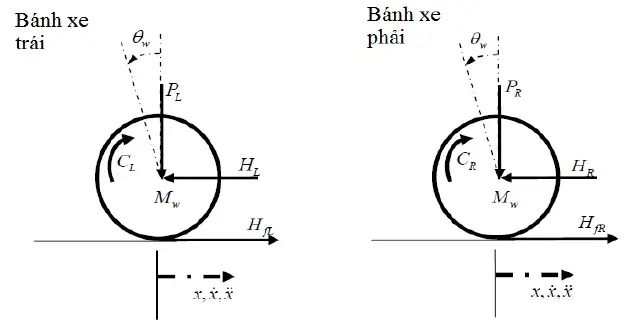
\includegraphics[width=1\textwidth]{pictures/wheel.png} 
            \caption{Sơ đồ tự do của các bánh}
        \end{figure}
        
        \hspace*{0.6cm}Áp dụng định luật 2 Newton cho phương ngang:
        \begin{align}
            \sum F_x &= M_w \ddot{x} = H_R - H_L 
        \end{align}
        
        Tổng moment quanh trọng tâm bánh xe:
        \begin{align}
            \sum M_o &= I_w \ddot{\theta} = C_R - H_R r 
        \end{align}
        
        Từ động học động cơ một chiều, moment quay động cơ được mô tả bởi:
        \begin{align}
            \tau_m = I_R \frac{d \omega}{dt} + \tau_a 
        \end{align}
        
        Với moment quay đầu ra:
        \begin{align}
            C = I_R \frac{d \omega}{dt} = -\frac{k_m k_e}{R} \dot{\theta}_w + \frac{k_m}{R} V_a 
        \end{align}
        
        Thay vào phương trình (1.2):
        \begin{align}
            I_w \ddot{\theta} = -\frac{k_m k_e}{R} \dot{\theta}_w + \frac{k_m}{R} V_a - H_R r 
        \end{align}
        
        Rút gọn biểu thức $H_R$:
        \begin{align}
            H_R = -\frac{k_m k_e}{Rr} \dot{\theta}_w  + \frac{k_m}{Rr} V_a - \frac{I_w}{r} \ddot{\theta}_w 
        \end{align}
        
        Phương trình (1.4) thay vào (1.1), ta thu được phương trình cho các bánh:
        
        \subsection*{Bánh xe bên trái}
            \begin{align}
                M_w \ddot{x} = -\frac{k_m k_e}{Rr} \dot{\theta}_w + \frac{k_m}{Rr} V_a - \frac{I_{w}}{r} \ddot{\theta}_w - H_L 
            \end{align}
        
        \subsection*{Bánh xe bên phải}
            \begin{align}
                M_w \ddot{x} = -\frac{k_m k_e}{Rr} \dot{\theta}_w  + \frac{k_m}{Rr} V_a - \frac{I_{w}}{r} \ddot{\theta}_w - H_R 
            \end{align}
        
        Bởi vì chuyển động tuyến tính được xem xét ở trọng tâm của bánh xe, góc quay có thể được biến đổi thành chuyển động tuyến tính bằng biến đổi đơn giản:
        \begin{align*}
            \ddot{\theta}_w r &= \ddot{x} \Rightarrow \ddot{\theta}_w = \frac{\ddot{x}}{r} \\
            \dot{\theta}_w r &= \dot{x} \Rightarrow \dot{\theta}_w = \frac{\dot{x}}{r}
        \end{align*}
       
        Bằng phép biến đổi tuyến tính, phương trình (1.7) và (1.8) có thể được viết lại như sau:
        \subsection*{Bánh xe bên trái}
        \begin{align}
            M_w \ddot{x} = -\frac{k_m k_e}{Rr^2} \dot{x} + \frac{k_m}{Rr^2} V_a - \frac{I_{w}}{r^2} \ddot{x} - H_L 
        \end{align}
        \subsection*{Bánh xe bên phải}
        \begin{align}
            M_w \ddot{x} = -\frac{k_m k_e}{Rr^2} \dot{x} + \frac{k_m}{Rr^2} V_a - \frac{I_{w}}{r^2} \ddot{x} - H_R 
        \end{align}
        \hspace*{0.6cm}Cộng 2 phương trình (1.9) và (1.10):
        \begin{align}
            2(M_w + \frac{I_w}{r^2})\ddot{x} = -\frac{2k_m k_e}{Rr^2} \dot{x} + \frac{2k_m}{Rr} V_a  - (H_L + H_R)
        \end{align}
    \section{Mô hình con lắc ngược}
        \hspace*{0.6cm}Cấu hình robot có thể được mô hình như một con lắc ngược
            \begin{figure}[H]
                \centering
                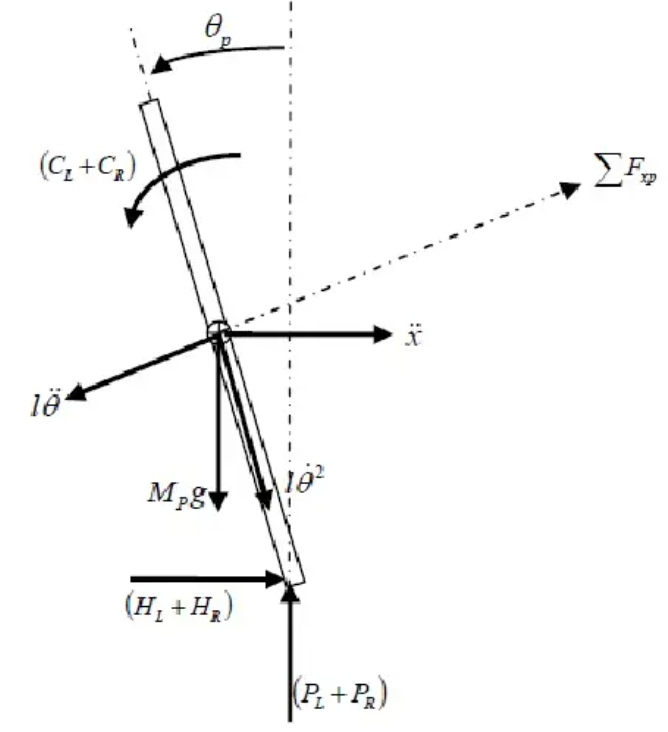
\includegraphics[width=0.5\textwidth]{pictures/inverted_pendulum.png} 
                \caption{Sơ đồ tự do của con lắc ngược}
            \end{figure}
        \subsection{Thiết lập hệ phương trình phi tuyến}
            Lặp lại, bằng việc sử dụng định luật 2 Newton, tổng các lực theo phương ngang:
            \begin{align}
                \sum F_x &= M_p \ddot{x} \nonumber\\
                (H_L + H_R) - M_p l \ddot{\theta} \cos &\theta_p + M_p l \dot{\theta}^2 \sin \theta_p = M_p \ddot{x} 
            \end{align}
            
            Suy ra:
            \begin{align}
                (H_L + H_R) &= M_p \ddot{x} + M_p l \ddot{\theta} \cos \theta_p - M_p l \dot{\theta}^2 \sin \theta_p 
            \end{align}
            
            Tổng các lực vuông góc với con lắc:
            \begin{align}
                \sum F_{xp} &= M_p \ddot{x} \cos \theta_p \nonumber\\
                (H_L + H_R) \cos \theta_p + (P_L + P_R) \sin& \theta_p - M_p g \sin \theta_p - M_p l \ddot{\theta}_p = M_p \ddot{x} \cos \theta_p 
            \end{align}
            
            Tổng moment quanh trọng tâm con lắc:
            \begin{align}
                \sum M_0 &= I_p a \nonumber \\
                -(H_L + H_R) l \cos \theta_p - (P_L + P_R) l&    \sin \theta_p - (C_L + C_R) = I_p \ddot{\theta} 
            \end{align}
            
            Moment quay áp dụng lên con lắc từ động cơ:
            \begin{align*}
                C_L + C_R = -\frac{2k_m k_e}{R} \frac{\dot{x}}{r} + \frac{2k_m}{R} V_a 
            \end{align*}
            
            Thay vào (1.15):
            \begin{align*}
                -(H_L + H_R) l \cos \theta_p - (P_L + P_R) l \sin \theta_p + \frac{2k_m k_e}{R} \frac{\dot{x}}{r} - \frac{2k_m}{R} V_a = I_p \ddot{\theta}_{p} 
            \end{align*}

            Do đó:
            \begin{align}
                -(H_L + H_R) l \cos \theta_p - (P_L + P_R) l \sin \theta_p = I_p \ddot{\theta}_{p} - \frac{2k_m k_e}{R} \frac{\dot{x}}{r} + \frac{2k_m}{R} V_a
            \end{align}

            Nhân phương trình (1.14) với $-l$ ta có:
            \begin{align*}
                -(H_L + H_R) l \cos \theta_p - (P_L + P_R) l \sin \theta_p + M_p g l \sin \theta_p + M_p l^2 \ddot{\theta}_p = -M_p l \ddot{x} \cos \theta_p 
            \end{align*}

            Thay thế phương trình (1.15) vào phương trình (1.16), ta được:

            \begin{equation}
                I_p \ddot{\theta}_p - \frac{2k_m k_e}{R} \frac{\dot{x}}{r} - \frac{2k_m}{R} V_a + M_p g l \sin\theta_p + M_p l^2 \ddot{\theta}_p = -M_p l \ddot{x} \cos\theta_p
            \end{equation}

            Để loại bỏ thành phần động học của động cơ \( (H_L + H_R) \), ta thay phương trình (1.13) vào phương trình (1.11), thu được:

            \begin{equation}
                2\left(M_w + \frac{I_w}{r^2} \right) \ddot{x} = -\frac{2k_m k_e}{R r^2} \dot{x} + \frac{2k_m}{R r} V_a - M_p \ddot{x} - M_p l \ddot{\theta}_p \cos\theta_p + M_p l \dot{\theta}_p^2 \sin\theta
            \end{equation}

            Kết hợp hai phương trình (1.17) và (1.18), ta có hệ phương trình chuyển động phi tuyến:

            \begin{align}
                (I_p +& M_p l^2)  \ddot{\theta}_p - \frac{2k_m k_e}{R r^2} \dot{x} + \frac{2k_m}{R r} V_a + M_p g l \sin\theta_p = -M_p l \ddot{x} \cos\theta_p  \\
                \frac{2k_m}{R r} V_a &= \left(2 M_w + \frac{2 I_w}{r^2} + M_p \right) \ddot{x} - \frac{2k_m k_e}{R r^2} \dot{x} + M_p l \ddot{\theta}_p \cos\theta_p - M_p l \dot{\theta}_p^2 \sin\theta_p 
            \end{align}

        \subsection{Tuyến tính hóa hệ phương trình}

            \hspace*{0.6cm}Để đơn giản và áp dụng điều khiển, ta giả sử:

            \[
            \theta_p = \pi + \phi
            \]

            Với \( \phi \) là một góc nhỏ so với phương thẳng đứng (tức là hệ đang dao động quanh vị trí thẳng đứng). Khi đó, các xấp xỉ tuyến tính:

            \[
            \cos\theta_p \approx -1, \quad \sin\theta_p \approx -\phi, \quad \left( \frac{d\theta_p}{dt} \right)^2 \approx 0
            \]

            Được áp dụng để đơn giản hóa hệ phương trình.

            Phương trình tuyến tính hóa của chuyển động là:

            \begin{equation}
                (I_p + M_p l^2)\ddot{\phi} - \frac{2k_m k_e}{R r} \dot{x} + \frac{2k_m}{R} V_a - M_p g l \sin \theta_p = M_p l \ddot{x}
            \end{equation}

            \begin{equation}
                \frac{2k_m}{R r} V_a = \left( 2M_w + \frac{2I_w}{r^2} + M_p \right) \ddot{x} + \frac{2k_m k_e}{R r^2} \dot{x} - M_p l \ddot{\phi}
            \end{equation}

            Để đưa hai phương trình trên về dạng phục vụ xây dựng mô hình không gian trạng thái, ta biến đổi:

            \begin{align}
                \ddot{\phi} &= \frac{M_p l}{(I_p + M_p l^2)} \ddot{x}
                + \frac{2k_m k_e}{R r (I_p + M_p l^2)} \dot{x}
                + \frac{2k_m}{R (I_p + M_p l^2)} V_a
                - \frac{M_p g l}{(I_p + M_p l^2)} \phi
                \\[1ex]
                \ddot{x} &= \frac{2k_m}{R r \left( 2M_w + \frac{2I_w}{r^2} + M_p \right)} V_a
                - \frac{2k_m k_e}{R r^2 \left( 2M_w + \frac{2I_w}{r^2} + M_p \right)} \dot{x}
                - \frac{M_p l}{\left( 2M_w + \frac{2I_w}{r^2} + M_p \right)} \ddot{\phi}
            \end{align}

            Nếu bỏ qua các thành phần quán tính kênh (ví dụ như động cơ), ta được:

            \begin{align}
                \ddot{\phi} + \frac{M_p g l}{I_p + M_p l^2} \phi &= \frac{2k_m}{R (I_p + M_p l^2)} V_a  \\[1ex]
                \ddot{x} + \frac{2k_m k_e}{(2M_w + \frac{2I_w}{r^2}) R^2} \dot{x} &= \frac{2k_m}{(2M_w + \frac{2I_w}{r^2}) R r} V_a
            \end{align}

            \noindent
            \hspace*{0.6cm}Trong mô hình này, giả thiết rằng bánh xe luôn tiếp xúc với mặt đất và không có trượt. Các lực quay và ma sát được bỏ qua.

            \subsection{Mô hình không gian trạng thái}

            \hspace*{0.6cm}Từ các phương trình đã tuyến tính hoá, ta xây dựng hệ phương trình không gian trạng thái dưới dạng:

            \begin{equation}
                \begin{bmatrix}
                    \dot{\phi} \\
                    \ddot{\phi}
                \end{bmatrix}
                =
                \begin{bmatrix}
                    0 & 1 \\
                    -\dfrac{M_p g l}{I_p + M_p l^2} & 0
                \end{bmatrix}
                \begin{bmatrix}
                    \phi \\
                    \dot{\phi}
                \end{bmatrix}
                +
                \begin{bmatrix}
                    0 \\
                    \dfrac{2k_m}{(I_p + M_p l^2) R}
                \end{bmatrix}
                 V_a
            \end{equation}

            \begin{equation}
                \begin{bmatrix}
                    \dot{x} \\
                    \ddot{x}
                \end{bmatrix}
                =
                \begin{bmatrix}
                    0 & 1 \\
                    0 & -\dfrac{2k_m k_e}{(2M_w + \frac{2I_w}{r^2}) R^2}
                \end{bmatrix}
                \begin{bmatrix}
                    x \\
                    \dot{x}
                \end{bmatrix}
                +
                \begin{bmatrix}
                    0 \\
                    \dfrac{2k_m}{(2M_w + \frac{2I_w}{r^2}) R r}
                \end{bmatrix}
                V_a
            \end{equation}
    \section{Hàm truyền hệ thống}

        \hspace*{0.6cm}Phương trình vi phân bậc hai của hệ được viết lại như sau:
        
        \begin{equation}
            \ddot{\phi} + \frac{M_p g l}{I_p + M_p l^2} \phi = \frac{2k_m}{R (I_p + M_p l^2)} V_a
        \end{equation}
        
        Gọi:
        
        \[
            x_1(t) = \phi(t), \quad x_2(t) = \dot{\phi}(t)
        \]
        
        Khi đó hệ phương trình trở thành:
        
        \[
        \begin{cases}
            \dot{x}_1(t) = x_2(t) \\
            \dot{x}_2(t) = -\frac{M_p g l}{I_p + M_p l^2} x_1(t) + \frac{2k_m}{R (I_p + M_p l^2)} V_a
        \end{cases}
        \]
        
        Biểu diễn dưới dạng ma trận không gian trạng thái:
        
        \begin{equation}
        \begin{bmatrix}
            \dot{x}_1(t) \\
            \dot{x}_2(t)
        \end{bmatrix}
        =
        \begin{bmatrix}
            0 & 1 \\
            -\frac{M_p g l}{I_p + M_p l^2} & 0
        \end{bmatrix}
        \begin{bmatrix}
            x_1(t) \\
            x_2(t)
        \end{bmatrix}
        +
        \begin{bmatrix}
            0 \\
            \frac{2k_m}{R (I_p + M_p l^2)}
        \end{bmatrix}
        V_a
        \end{equation}
        
        Với đầu ra \( y(t) = \phi(t) = x_1(t) \Rightarrow \)
        
        \[
        y(t) = \begin{bmatrix} 1 & 0 \end{bmatrix}
        \begin{bmatrix}
            x_1(t) \\
            x_2(t)
        \end{bmatrix}
        \]
        
        \textbf{Giá trị các thông số:}
        \[
            M_p = 1.2 \, \text{kg}, \quad g = 9.81, \quad l = 0.1, \quad I_p = 0.01, \quad k_m = 0.28, \quad R = 5.25 \, \Omega
        \]
        
        Thay số vào ta có ma trận hệ:
        
        \[
            A = \begin{bmatrix} 0 & 1 \\ -53.51 & 0 \end{bmatrix}, \quad
            B = \begin{bmatrix} 0 \\ 4.85 \end{bmatrix}, \quad
            C = \begin{bmatrix} 1 & 0 \end{bmatrix}, \quad
            D = 0
        \]
        
        Từ mô hình không gian trạng thái, ta có:
        
        \[
        G(s) = C(sI - A)^{-1}B
        \]
        
        Tính:
        
        \[
        sI - A =
        \begin{bmatrix}
            s & -1 \\
            -53.51 & s
        \end{bmatrix}, \quad
            (sI - A)^{-1} = \frac{1}{s^2 + 3.51}
        \begin{bmatrix}
            s & 1 \\
            -53.51 & s
        \end{bmatrix}
        \]
        
        Do đó:
        
        \begin{align*}
            G(s) &= \begin{bmatrix} 1 & 0 \end{bmatrix}
            \cdot \frac{1}{s^2 + 53.51}
        \begin{bmatrix}
            s & 1 \\
            -53.51 & s
        \end{bmatrix}
        \cdot
        \begin{bmatrix}
            0 \\
            4.85
        \end{bmatrix} \\
        &= \frac{1}{s^2 + 3.51} \cdot \begin{bmatrix} 1 & 0 \end{bmatrix}
        \cdot
        \begin{bmatrix}
            4.85
        \end{bmatrix}
        = \frac{1.85}{s^2 + 53.51}
        \end{align*}
        
        \textbf{Vậy:}
        \[
            G(s) = \frac{4.85}{s^2 + 53.51}
        \]
        
        Đây là hàm truyền từ điện áp điều khiển \( V_a \) đến góc lệch \( \phi(t) \) của con lắc ngược.
    \section{Kết luận}
        Sau khi thực hiện quá trình mô hình hóa, tuyến tính hóa và xây dựng hệ phương trình không gian trạng thái, ta đã thu được hàm truyền tuyến tính biểu diễn mối quan hệ giữa điện áp điều khiển đầu vào $V_a$ và góc nghiêng $\phi$ của robot hai bánh:

        \[
        G(s) = \frac{4.85}{s^2 + 53.51}
        \]
        
        Hàm truyền trên cho thấy hệ thống là một hệ dao động bậc hai không có thành phần tắt dần (damping) và có tính chất **marginally stable** (ổn định biên). Điều này là đặc trưng của mô hình con lắc ngược: hệ không ổn định khi không có điều khiển tác động.
        
        Việc xây dựng được hàm truyền là một bước quan trọng, tạo nền tảng để thiết kế các bộ điều khiển như PID, LQR hoặc các chiến lược điều khiển hiện đại nhằm đảm bảo robot giữ được trạng thái cân bằng và theo dõi quỹ đạo mong muốn.
        
        Trong chương tiếp theo, ta sẽ tiến hành thiết kế và mô phỏng các bộ điều khiển dựa trên hàm truyền đã thu được.
            
        
       
    \chapter{KHẢO SÁT TÍNH ỔN ĐỊNH CỦA HỆ THỐNG}
    Ta có hàm truyền đã tìm được ở trên là:
    \[
        G(s) = \frac{4.85}{s^2 + 53.51}
    \]
    Hệ vòng kín với phản hồi là: 
    \[
        T(s) = \frac{G(s)}{1+G(s)} 
    \]
    Phương trình đặc tính:
    \begin{align*}
        &1 + G(s) = 0 \\
        &\Leftrightarrow 1 + \frac{4.85}{s^2 + 53.51} = 0 \\
        &\Leftrightarrow s^2 + 58.36 = 0
    \end{align*}
    $\Leftarrow$ Hệ không ổn định do hệ số của $s^1$ là 0. 
    \section{Biểu đồ Bode}
    \[
        G(s) = \frac{4.85}{s^2 + 53.51}
    \]
    Phân tích:
    \begin{itemize}
        \item 1 khâu khuếch đại: K = 4.85.
        \item 1 khâu dao động bậc 2.
    \end{itemize}
    Tần số cộng hưởng: 
    \[
        \omega_n = \sqrt{53.51} = 7.315 (rad/s)
    \]
    Đặc tính tần số:
    \[
        G_1(j\omega) = \frac{4.85}{-\omega^2 + 53.51}
    \]
    \textbf{Biên độ:}
    \[
        M(\omega) = \abs{G(j\omega)} = \frac{4.85}{\abs{-\omega^2 + 53.51}}
    \]
    \[
        \Rightarrow L(\omega) = 20log(M(\omega)) = 20log(4.85) - 20log(\abs{-\omega^2 + 53.51})
    \]
    \begin{itemize}
        \item Khi $0<\omega<7.315$: biên độ tăng từ -20.85dB đến $+\infty$
        \item Với $\omega > 7.315$: 
    \end{itemize}
    \begin{align*}
        &20log(4.85) - 20log(\abs{-\omega^2 + 53.51}) \approx 20log(4.85) - 20log(\omega^2) \\
        &= 20log(4.85) - 40log(\omega) \\
        &\Rightarrow \text{Độ dốc giảm: } -40dB/decade \\
        &\Rightarrow \text{Với } \omega > 7.315: \text{ biên độ giảm từ } +\infty \text{ về } -\infty
    \end{align*}
    \textbf{Pha:}
    \begin{itemize}
        \item $\omega < 7.314$: $-\omega^2 + 53.509 > 0$, pha $\angle G_1(j\omega) = 0^\circ$,
        \item $\omega = 7.314$: $-\omega^2 + 53.509 = 0$, pha nhảy từ $0^\circ$ xuống $-180^\circ$,
        \item $\omega > 7.314$: $-\omega^2 + 53.509 < 0$, pha $\angle G_1(j\omega) = -180^\circ$.
    \end{itemize}
    \textbf{Tính độ dự trữ biên độ (GM):}
    \begin{itemize}
        \item \textbf{Tìm tần số cắt pha} ($\omega_{pc}$): Đây là tần số mà pha đạt $-180^\circ$.
        \begin{itemize}
            \item Từ phân tích pha, $\angle G_1(j\omega) = -180^\circ$ khi $\omega \geq 7.314$.
            \item Vậy $\omega_{pc} = 7.314$ rad/s.
        \end{itemize}
        \item \textbf{Tính biên độ tại $\omega_{pc}$:}
            \[
            |G_1(j\omega_{pc})| = \left| \frac{4.848}{-(7.314)^2 + 53.509} \right| = \frac{4.848}{0} \to \infty
            \]
            \[
            |G_1(j\omega_{pc})|_{dB} \to +\infty \text{ dB}
            \]
            \item \textbf{Độ dự trữ biên độ:}
            \[
            \text{GM (dB)} = -20 \log_{10} |G_1(j\omega_{pc})| \to -\infty \text{ dB}
            \]
    \end{itemize}
    \textbf{Tính độ dự trữ pha ($\phi_M$):}           
        \begin{itemize}
            \item \textbf{Tìm tần số cắt biên độ} ($\omega_{gc}$): Đây là tần số mà $|G_1(j\omega)| = 1$ (0 dB).
            \begin{itemize}
                \item Đặt $|G_1(j\omega)| = 1$:
                \[
                \left| \frac{4.848}{-\omega^2 + 53.509} \right| = 1
                \]
                \item Khi $\omega < 7.314$, $|-\omega^2 + 53.509| = 53.509 - \omega^2$, nên:
                \begin{align*}
                    \frac{4.848}{53.509 - \omega^2} = 1 \Rightarrow 53.509 - \omega^2 = 4.848 \\
                    \Rightarrow \omega^2 = 53.509 - 4.848 = 48.661 \\
                    \Rightarrow \omega_{gc} \approx \sqrt{48.661} \approx 6.976 \, \text{rad/s}
                    \end{align*}
                \end{itemize}
                \item \textbf{Tính pha tại $\omega_{gc}$:} \\
                    Tại $\omega_{gc} = 6.976 < 7.314$, pha $\angle G_1(j\omega_{gc}) = 0^\circ$.
                \item \textbf{Độ dự trữ pha:}
                \[
                \phi_M = 180^\circ + \angle G_1(j\omega_{gc}) = 180^\circ + 0^\circ = 180^\circ
                \]
            \end{itemize}
        
    \begin{figure}[H]
        \centering
        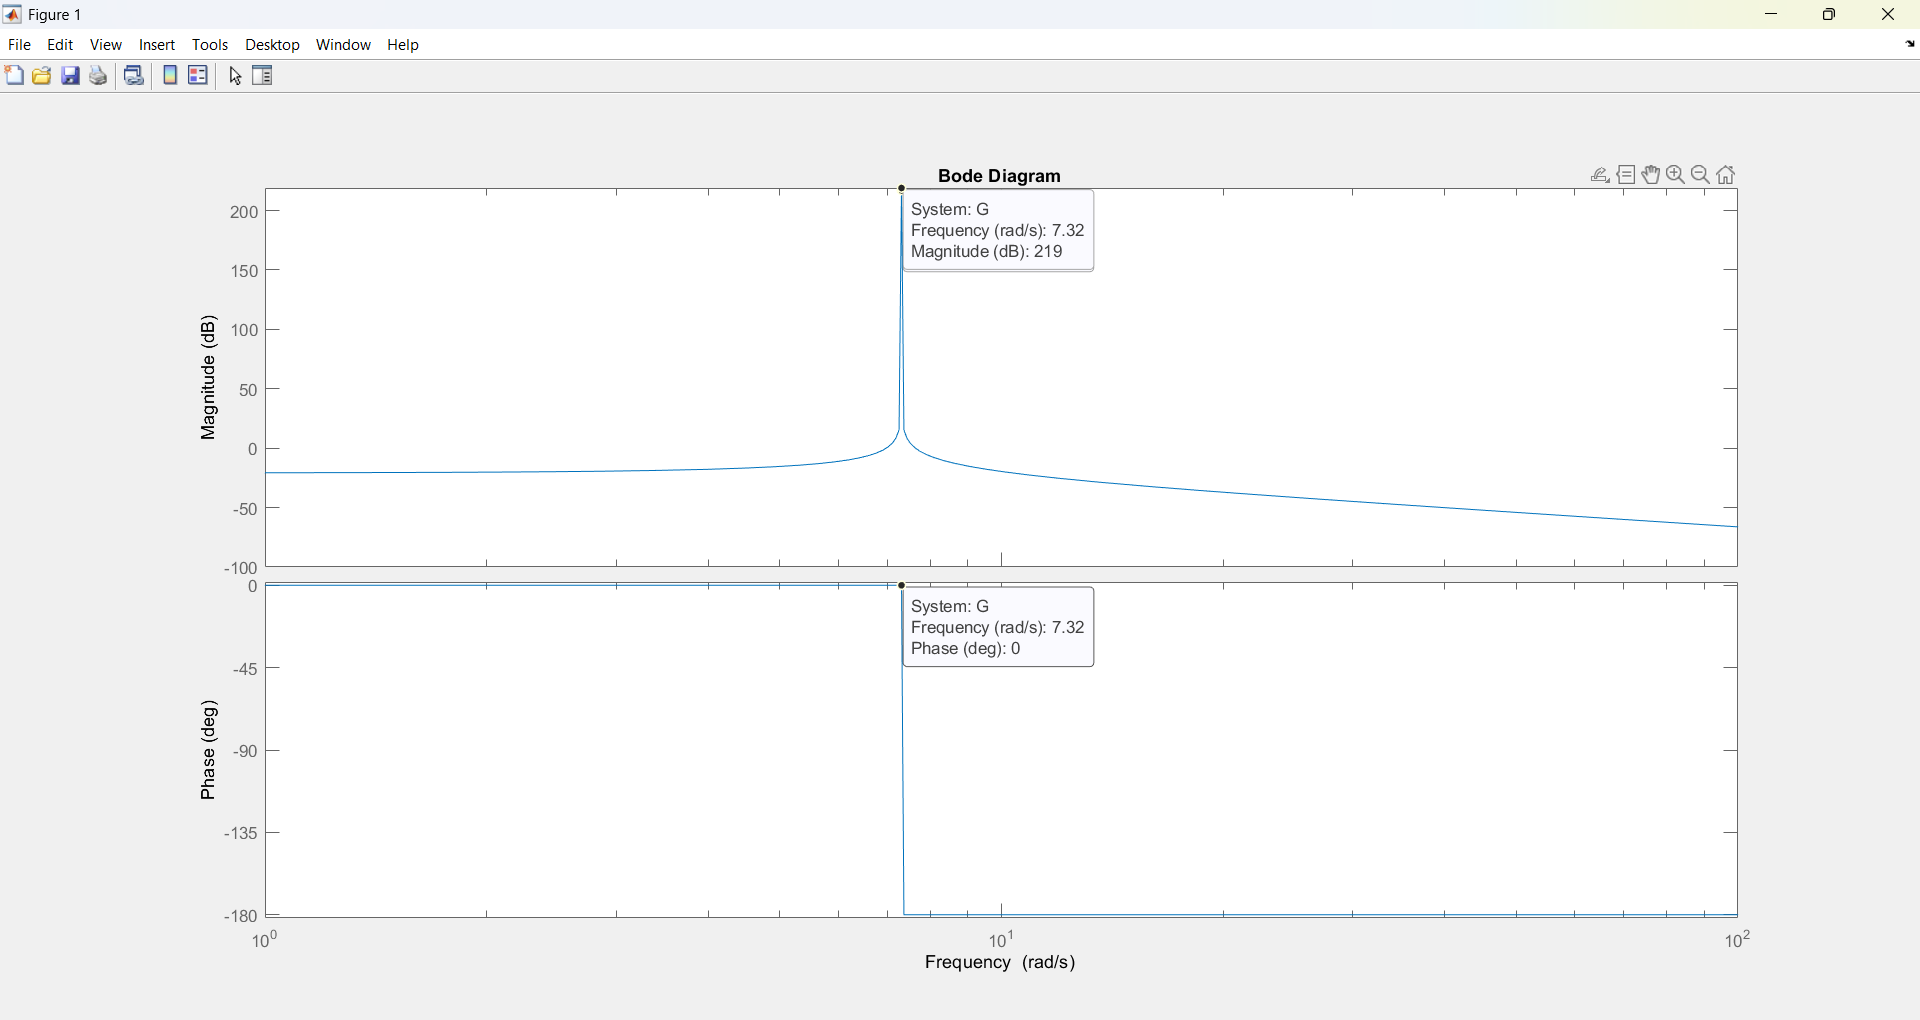
\includegraphics[width=1\textwidth]{pictures/bode.png}
    \end{figure}
    Nhận xét:
    \begin{itemize}
        \item Hệ thống vòng hở: G(s) có các cực trên trục ảo $s=+-7.315$ nên hệ thống ổn định biên. Đồ thị Bode cho thấy biên độ đạt đỉnh tại $\omega=7.315$ và pha nhảy xuống là $-180^\circ$. Điều này xác nhận hệ thống dao động không suy giảm.
        \item Từ độ thị ta có thể thấy độ dữ trữ pha $G_M < 0 dB$ nên đã vi phạm tiêu chuẩn ổn định của biểu đồ Bode $\Rightarrow$ Hệ chưa ổn định. 
    \end{itemize}

    % \chapter{ĐÁNH GIÁ CHẤT LƯỢNG HỆ THỐNG ĐIỀU KHIỂN}
\[
    G(s) = \frac{4.85}{s^2 + 53.51}
\]
\section{Các tiêu chuẩn về xác lập}
Hàm truyền vòng kín:
\[
    T(s) = \frac{G(s)}{1+G(s)} = \frac{4.85}{s^2 + 58.36}
\]
Xét với đầu vào bậc (step input, $R(s)=\frac{1}{s}$), sai số xác lập được tính bằng:
\[
e_{xl} = \lim_{s \to 0} \frac{s \cdot R(s)}{1 + G(s)} 
= \lim_{s \to 0} \frac{1}{1 + k_p} \approx 0{,}92
\]
\begin{center}
    Với $k_p$  là hệ số vị trí, $k_p = \lim_{s \to 0} G(s) \approx 0.09$ 
\end{center}
\textbf{Khảo sát hệ thống là bậc 2}
\begin{figure}[H]
    \centering
    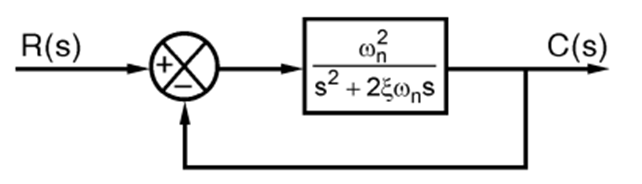
\includegraphics[width=0.8\textwidth]{pictures/closeloop.png}
\end{figure}

Hàm truyền hệ dao động bậc 2:
\[
    G_2(s) = \frac{K\omega^2}{s^2+2\zeta \omega s + \omega^2}
\]
Đáp ứng quá độ:
\[
    C(s) = R(s)\cdot G_2(s) = \frac{1}{s}\cdot \frac{K\omega^2}{s^2+2\zeta \omega s + \omega^2}
\]
$\Rightarrow$ Laplace ngược: 
\[
    c(t) = K\{1-\frac{e^{-\zeta \omega_n t}}{\sqrt{1-\zeta^2}}\cdot sin[(\omega_n\sqrt{1-\zeta^2})\cdot t+\theta] \}
\]
Qua đó ta thấy hệ dao động không giảm chấn với $\zeta = 0$.\\
Hệ dao động bậc 2 có 2 cặp cực phức: $p_{1,2} = \pm j\,7{,}639$ \\

\textbf{Từ đó xác định các thông số cơ bản }
\begin{itemize}
    \item Tần số tự nhiên: $\omega_n = 7{,}639$
    \item Hệ số giảm chấn: $\zeta = 0$
    \item Thời gian đạt đỉnh: $T_p = \frac{\pi}{\omega_n \sqrt{1 - \zeta^2}} = 0{,}411s$
    \item Độ vọt lố: $\text{POT} = e^{\frac{-\zeta \pi}{1-\zeta^2}} \cdot 100 = 100\%$
    \item Thời gian xác lập: Với tiêu chuẩn 2\% $\Rightarrow T_p = \frac{4}{\zeta \omega_n} \rightarrow \infty$
    \item Đáp ứng quá độ: $C(s) = R(s) \cdot T(s) = \frac{1}{s} \cdot \frac{4{,}85}{s^2 + 58{,}36}$
\end{itemize}
\[
\Rightarrow c(t) = \frac{4.85}{7.639^2} \left[1 - \sin(7.639 \cdot t + \frac{\pi}{2})\right] = 0.083 - 0.083 \cos(7.639 \cdot t)
\]
\begin{figure}[H]
    \centering
    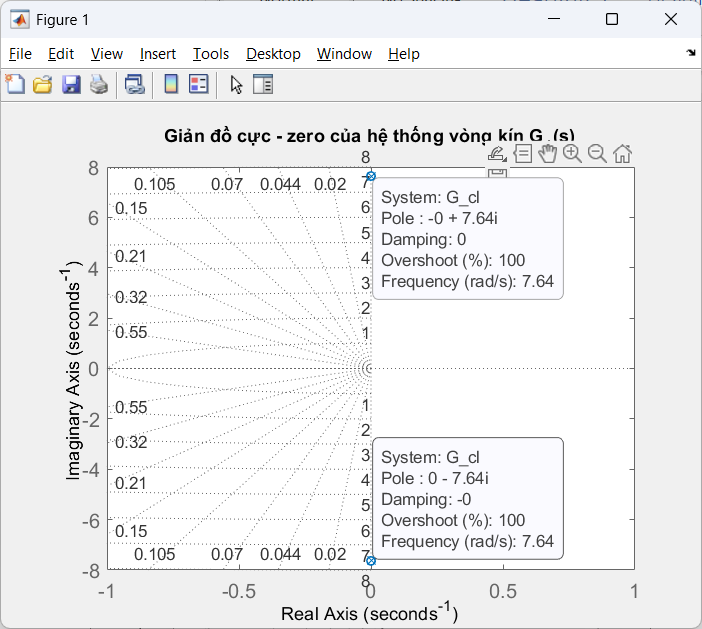
\includegraphics[width=0.8\textwidth]{pictures/poleszeros.png}
\end{figure}
\begin{figure}[H]
    \centering
    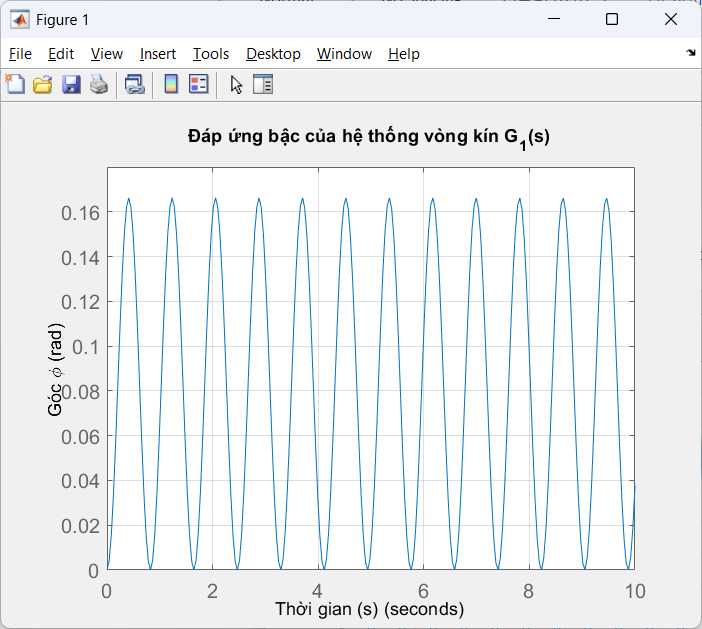
\includegraphics[width=0.8\textwidth]{pictures/step.png}
\end{figure}
\textbf{Nhận xét:} Đáp ứng quá độ của khâu dao động bậc 2 có dạng dao động với biên độ giảm dần.
Do $\zeta = 0$, đáp ứng của hệ là dao động không suy giảm với tần số tự nhiên $\omega_n = 7.639$.
    \chapter{THIẾT KẾ BỘ ĐIỀU KHIỂN CTC (Computed-Torque Control)}
    \section{Tiêu chí thiết kế}
    \hspace*{0.6cm}Tiêu chí thiết kế:
    \begin{itemize}
        \item Settling time: $T_s < 4\text{s}$
        \item Overshoot: \%OS < 10\%
    \end{itemize}

    Đối với hệ thống bậc 2, ta có:

    \[
    T_s = \frac{4}{\omega_n}, \quad \%OS = 100e^{\left(-\zeta\pi / \sqrt{1-\zeta^2}\right)}
    \]

    Hệ số giảm chấn $\zeta$ tính từ \%OS:

    \[
    \zeta = \frac{-\ln\left(\frac{\%OS}{100}\right)}{\sqrt{\pi^2 + \ln^2\left(\frac{\%OS}{100}\right)}} = 0.5911
    \]

    Chọn $\zeta = 0.7$

    Suy ra:

    \[
    \omega_n > \frac{4}{\zeta T_s} = \frac{4}{0.7 \cdot 4} = 1.42857
    \]

    Chọn $\omega_n = 1.5 \text{ (rad/s)}$

    \section{Computed-Torque Control}
            Từ hệ phương trình (1.16), ta đưa về dạng tổng quát
            \begin{equation}
                M(q) \ddot{q} + C (q, \dot{q}) \dot{q} + G(q) = \tau
            \end{equation}
            Trong đó
            \begin{itemize}
                \item $q = [x \,\, \theta]^T$: vector trạng thái
                \item $M(q)$: ma trận quán tính
                \item $C(q, \dot{q})$: ma trận Coriolis và ly tâm
                \item $G(q)$: vector trọng lực
                \item $\tau$: moment xoắn điều khiển từ động cơ
            \end{itemize} 
            Ta được
            \begin{align*}
                &\underbrace{
                \begin{bmatrix}
                M_\Sigma & M_p \ell \cos \theta\\
                M_p \ell  \cos \theta & J
                \end{bmatrix}
                }_{M(q)}
                \begin{bmatrix}
                \ddot{x} \\ \ddot{\theta}
                \end{bmatrix}
                +
                \underbrace{
                \begin{bmatrix}
                0 & -M_p \ell \dot{\theta} \sin \theta \\
                0 & 0
                \end{bmatrix}
                }_{C(q, \dot{q})}
                \begin{bmatrix}
                \dot{x} \\ \dot{\theta}
                \end{bmatrix} 
                +
                \underbrace{
                \begin{bmatrix}
                0 & 0 \\
                0 & -M_p g \ell \sin \theta
                \end{bmatrix}
                }_{G(q)}
                =
                \underbrace{
                \begin{bmatrix}
                F_x \\
                \tau
                \end{bmatrix}
                }
            \end{align*}
        Định nghĩa lỗi theo dõi
        \begin{align}
            &e(t) = q_d(t) - q(t) \nonumber \\
            &\dot{e}(t) = \dot{q}_d(t) - \dot{q}(t) \nonumber \\
            &\ddot{e}(t) = \ddot{q}_d(t) - \ddot{q}(t) \nonumber
        \end{align}
        Ta có thể viết lại
        \begin{align}
            \ddot{e} = \ddot{q}_d(t) + M^{-1} (C(q, \dot{q})\dot{q} + G(q) - \tau)  \nonumber
        \end{align}
        Đặt tín hiệu điều khiển $u$ trở thành
        \begin{align}
            u = \ddot{q}_d(t) + M^{-1} (C(q, \dot{q})\dot{q} + G(q) - \tau)  
        \end{align}
        Ở đây giả sử cho nhiễu môi trường 
        \begin{align*}
            \tau_d = 0
        \end{align*}
        Khi đó 
        \begin{align*}
            \ddot{e} = u
        \end{align*}
        Từ phương trình (2.1), moment xoắn đầu ra được tính như sau
        \begin{align}
            \tau = M(q)(\ddot{q_d} - u) + C(q, \dot{q})\dot{q} + G(q)
        \end{align}         
        Giả sử chọn $u$ như là một bộ điều khiển PD, ta có
        \begin{align*}
            u = - K_p e - K_d \dot{e}
        \end{align*}
        Với $K_p$ và $K_d$ là ma trận điều khiển tỉ lệ và vi phân tương ứng. Khi đó phương trình (2.3) trở thành
        \begin{align}
            \tau = M(q)(\ddot{q_d} + K_p e + K_d \dot{e}) + C(q, \dot{q})\dot{q} + G(q)
        \end{align} 
        Phương trình vòng kín của lỗi động lực học
        \begin{align}
            \ddot{e} + K_p e + K_d \dot{e} = 0
        \end{align}
        Trong không gian trạng thái
        \begin{align*}
            \frac{d}{dt}
            \begin{bmatrix}
            e \\ \dot{e}
            \end{bmatrix}
            =
            \begin{bmatrix}
            0 & I \\
            -K_p & -K_d
            \end{bmatrix}
            \begin{bmatrix}
            e \\ \dot{e}
            \end{bmatrix}
        \end{align*}
        Phương trình đặc trưng
        \begin{align*}
            s^2 + K_d s + K_p = 0
        \end{align*}
        Có dạng chuẩn theo yêu cầu thiết kế
        \begin{align*}
            s^2 + 2\zeta \omega_n s + \omega_n^2 = 0
        \end{align*}
        So sánh ta thu được
        \begin{equation*}
            \begin{cases}
                K_d = 2\zeta \omega_n  = 2 \cdot 0.7 \cdot 1.5 = 2.1\\
                K_p = \omega_n^2 = 1.5^2 = 2.25
            \end{cases}
        \end{equation*}
        Đồ thị đáp ứng của vị trí góc (ban đầu góc $-\dfrac{\pi}{2}$, tức là ban đầu xe nằm ngang)
        \begin{figure}[H]
            \centering
            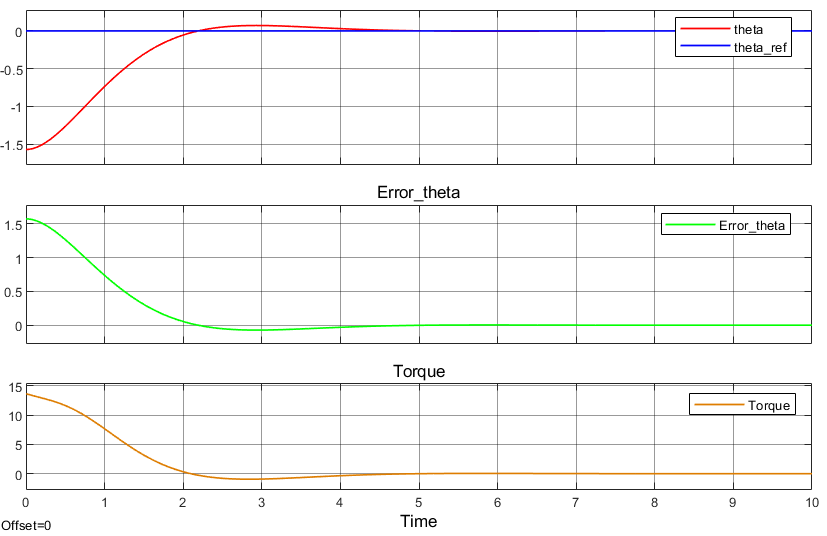
\includegraphics[width=1\textwidth]{pictures/torce.png}
            \caption{Đáp ứng vị trí góc}
        \end{figure}
        Đồ thị đáp ứng của vị trí
        \begin{figure}[H]
            \centering
            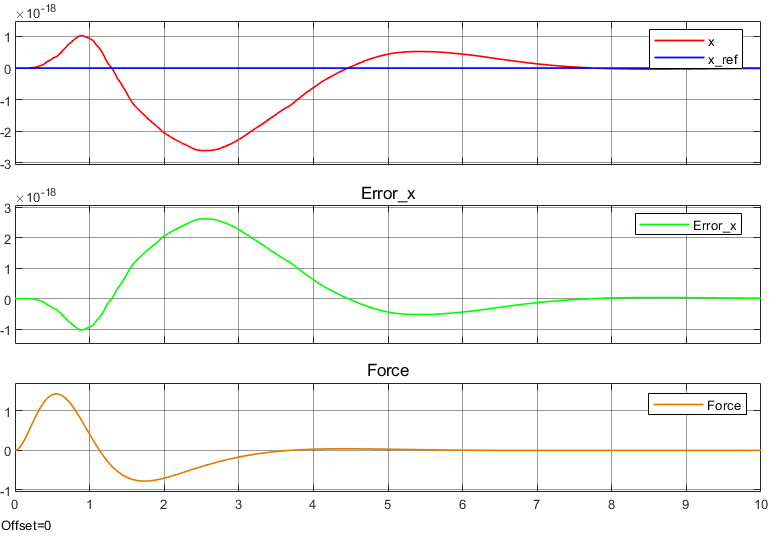
\includegraphics[width=1\textwidth]{pictures/force.png}
            \caption{Đáp ứng vị trí}
        \end{figure}
    \makeatletter
    \renewcommand{\appendixname}{Phụ lục}         % Dùng cho tiêu đề trong trang chương
    \renewcommand{\appendixtocname}{Phụ lục}       % Dùng cho tiêu đề trong Mục lục
    \renewcommand{\@chapapp}{Phụ lục}              % Dùng cho 'Phụ lục A', 'Phụ lục B'
    \makeatother
    \begin{appendices}
        \chapter{Code matlab}
    \section{Sơ đồ hệ thống điều khiển}
    \begin{figure}[H]
        \centering
        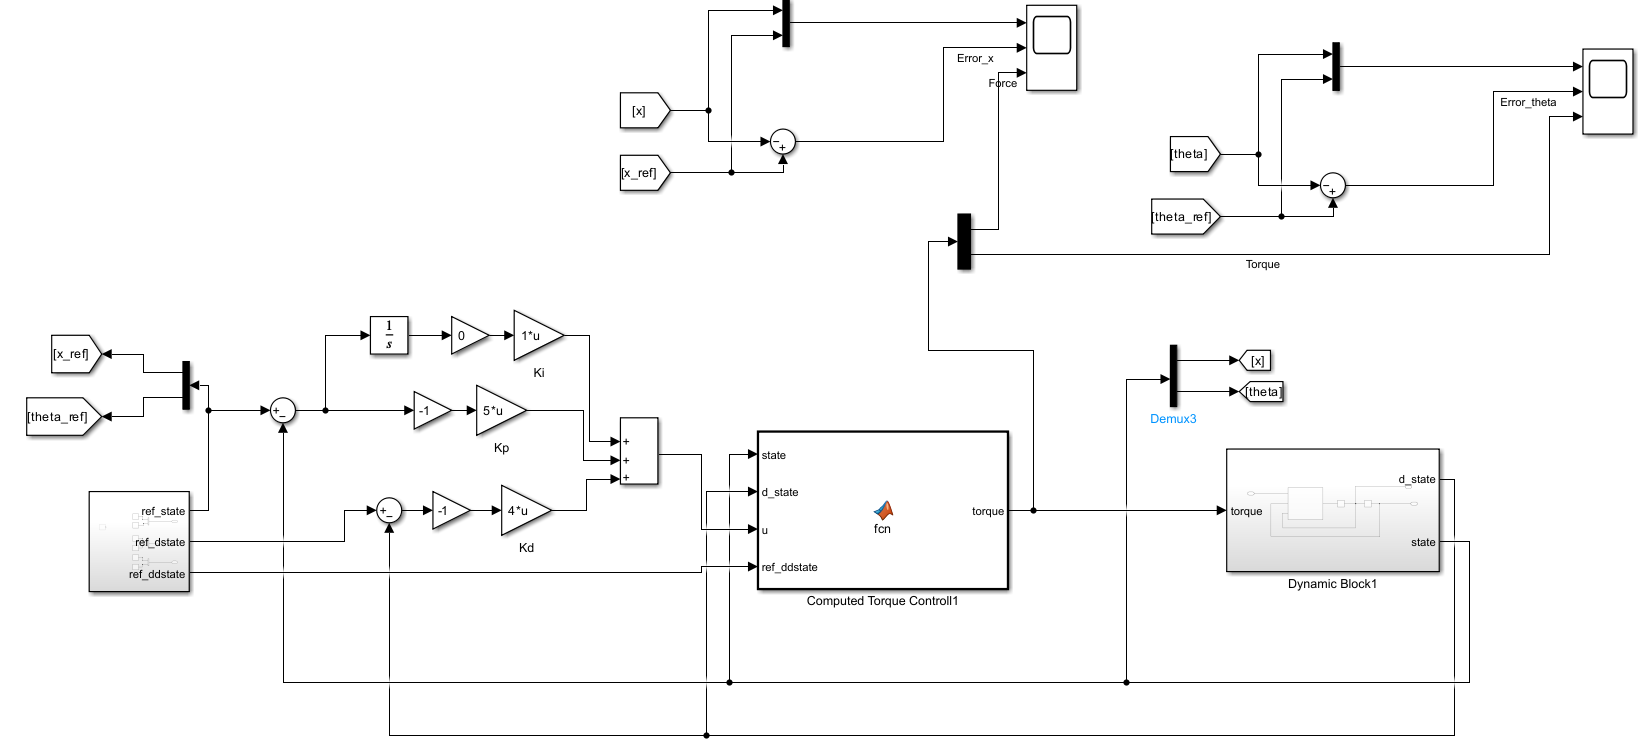
\includegraphics[width=1\textwidth]{pictures/ctc.png}
        \caption{Sơ đồ chung hệ thống điều khiển CTC}
    \end{figure}

    \section{Khối Dynamics}
    \begin{figure}[H]
        \centering
        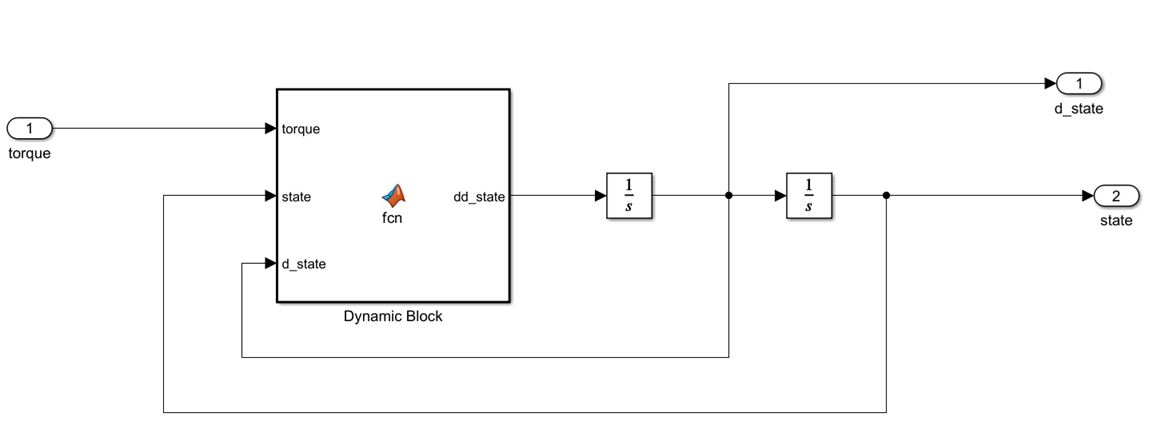
\includegraphics[width=1\textwidth]{pictures/dynamic_ctc.png}
    \end{figure}
    \begin{lstlisting}[caption={Code khối Dynamic Block}, label={lst:pz}]
        function dd_state = fcn(torque, state, d_state)
            % Define constant
            g = 9.81;
            r = 0.077;
            Mw = 0.3;
            Mp = 6;
            Iw = 0.0017;
            Ip = 0.29;
            l = 0.2;
            km = 0.0458;
            ke = 0.0458;
            R = 2.49;
        
        
            % Define variables
            x = state(1);
            theta = state(2);
            dx = d_state(1);
            dtheta = d_state(2);
    
            % Compute dynamic matrix
            M = ... 
            [Mp + 2*Mw + (2*Iw)/r^2, Mp*l*cos(theta);
                Mp*l*cos(theta),     Mp*l^2 + Ip];
            
            C =... 
            [0, -Mp*dtheta*l*sin(theta);
            0,                       0];
            
            V =... 
            [-Mp*dtheta^2*l*sin(theta);
                                    0];
            
            G = ...
            [                 0;
            -Mp*g*l*sin(theta)];
            
            B = [2/r; -2];
            
            % Compute acceleration
            dd_state = inv(M)*(torque - G - V); 
    \end{lstlisting}


    \section{Khối Computed-Torque Control + Input}
    \begin{figure}[H]
        \centering
        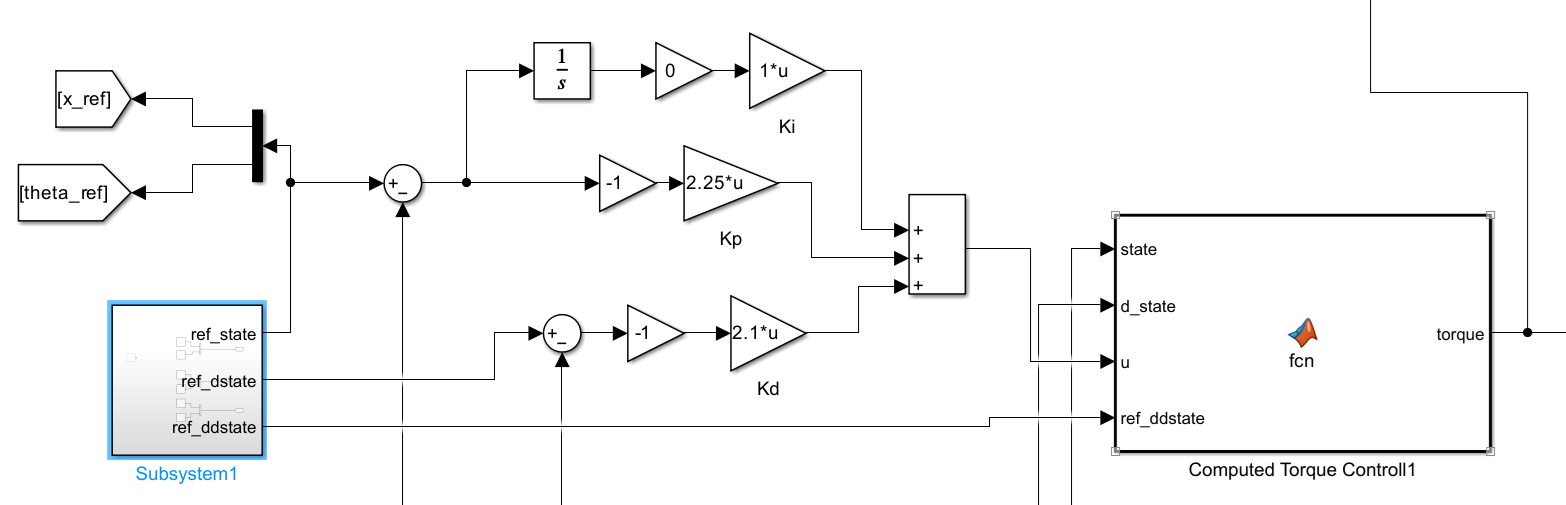
\includegraphics[width=1\textwidth]{pictures/ref_ctc.png}
    \end{figure}
    \begin{lstlisting}[caption={Code khối Computed-Torque Control}, label={lst:step}]
        function torque = fcn(state, d_state, u, ref_ddstate)
        % Define constant
        g = 9.81;
        r = 0.077;
        Mw = 0.3;
        Mp = 6;
        Iw = 0.0017;
        Ip = 0.29;
        l = 0.2;
        km = 0.0458;
        ke = 0.0458;
        R = 2.49;     
        
        % Define variables
        x = state(1);
        theta = state(2);
        dx = d_state(1);
        dtheta = d_state(2);
               
        M = ... 
        [Mp + 2*Mw + (2*Iw)/r^2, Mp*l*cos(theta);
               Mp*l*cos(theta),     Mp*l^2 + Ip];        
         
        C =... 
        [0, -Mp*dtheta*l*sin(theta);
        0,                       0];
         
         
        V =... 
        [-Mp*dtheta^2*l*sin(theta);
                                0];
         
         
        G = ...
        [                 0;
        -Mp*g*l*sin(theta)];
        
        
        
        B = [2/r; -2];
        B_dagger = pinv(B); 
        
        %tau is scalar
        tau = B_dagger * (M *(ref_ddstate - u) + V + G);

        
        torque = (M*(ref_ddstate - u) + V + G);       
    \end{lstlisting}



    

    \end{appendices}
    
\end{document}